\documentclass[12pt,a4paper]{article}
\usepackage[utf8]{inputenc}
\usepackage[english,russian]{babel}
\usepackage{indentfirst}
\usepackage{misccorr}
\usepackage{graphicx}
\usepackage{amssymb}
\usepackage{amsmath}
\usepackage{wrapfig}

\begin{document}

\begin{center}
    \large
    Работа 2.1.3
    
    Сибгатуллин Булат, Б01-007
    
    \vspace{0.5cm}
    \textbf{Определение $C_p/C_v$ по скорости звука в газе}

\end{center}

\vspace{0.5cm}
\textbf{Цель работы:} 1) измерение частоты колебаний и длины волны при резонансе звуковых колебаний в газе, заполняющем трубу; 2) определение показателя адиабаты  с помощью уравнения состояния идеального газа.

\vspace{0.5cm}
\textbf{В работе используются:} звуковой генератор ГЗ; электронный осциллограф ЭО; микрофон; телефон; раздвижная труба; теплоизолированная труба, обогреваемая водой из термостата; баллон со сжатым углекислым гозом; газгольдер.

\vspace{0.5cm}

Скорость распространения звуковой волны в газах зависит от показателя адиабаты $\gamma$. На измерении скорости звука основан один из наиболее точных методов определения показателя адиабаты.

Скорость звука в газах определяется формулой:

\[c = \sqrt {\gamma \frac{RT}{\mu}},\]

где \textit{R} - газовая постоянная, \textit{T} - температура газа, а $\mu$ - его молярная масса. Преобразуя эту формулу, найдем

\begin{equation}\label{1}
\gamma = \frac{\mu}{RT} c^2
\end{equation}

Звуковая волна, распространяющаяся вдоль трубы, испытывает многократные отражения от торцов. Звуковые колебания в трубе являются наложением всех отраженных волн и, вообще говоря, очень сложны. Картина упрощается, если длина трубы \textit{L} равна целому числу полуволн, то есть когда

\begin{equation}\label{2}
L = n \frac{\lambda}{2},
\end{equation}

где $\lambda$ - длина волны звука в трубе, а \textit{n} - любое целое число. Если условия (\ref{2}) выполнено, то волна, отраженная от торца трубы, вернувшаяся к её началу и вновь отраженная, совпадает по фазе с падающей. Совпадающие по вазе волны усиливают друг друга. Амплитуда звуковых колебаний при этом резко возрастает - наступает резонанс.

При звуковых колебаниях слои газа, прилегающие к торцам трубы, не испытывают смещения (\textit{узел смещения}). Узлы смещения повторяются по всей длине трубы через $\lambda / 2$.между узлами находятся максимумы смещения (\textit{пучности}).

Скорость звука \textit{c} связана с его частотой \textit{f} и длиной волны $\lambda$ соотношением

\begin{equation}\label{3}
c = \lambda f.
\end{equation}

1. При неизменной частоте \textit{f} звукого генератора (а следовательно и неизменной длине звуковой волны $\lambda$) можно изменять длину трубы \textit{L}. Для этого применяется раздвижная труба. Длина раздвижной трубы постепенно увеличивается, и наблюдается ряд последовательных резонансов. Возникновение резонанса легко наблюдать на осциллографе по резкому увеличению амплитуды колебаний. Для последовательных резонансов имеем

\[L_{n+k} = n\frac{\lambda}{2} + k\frac{\lambda}{2},\]

т.е. $\lambda / 2$ равно угловому коэффициенту графика, изображающего зависимость длины трубы \textit{L} от номера резонанса \textit{k}. Скорость звука находится по формуле (\ref{3}).

2. При постоянной длине трубы можно изменять частоту звуковых колебаний.В этом случае следует плавно изменять частоту \textit{f} звукового генератора, а следовательно, и длину звуковой волны $\lambda$. Для последовательных резонансов получим

\begin{equation}\label{4}
L = \frac{\lambda_1}{2}n = ... = \frac{\lambda_{k+1}}{2}(n + k).
\end{equation}

Из (\ref{3}) и (\ref{4}) имеем

\[f_1 = \frac{c}{\lambda_1} = \frac{c}{2L}n, \: f_2 = \frac{c}{\lambda_2} = \frac{c}{2L}(n + 1) = f_1 + \frac{c}{2L}, \: ...,\]

\begin{equation}\label{5}
f_{k+1} = \frac{c}{\lambda_{k+1} = \frac{c}{2L} (n+k) = f_1 + \frac{c}{2L}k.}
\end{equation}

Скорость звука, деленная на $2L$, определяется, таким образом, по угловому коэффициенту графика зависимости частоты от номера резонанса.

\textbf{1.} Проведем измерения на 1 установке для углекислого газа и воздуха.

Для углекислого газа:

\begin{tabular}{|c|c|c|c|}
\hline 
$f_1 = 2909 \: \textit{Гц}$ & $f_2 = 2096 \: \textit{Гц}$ & $f_3 = 2506 \: \textit{Гц}$ & $f_4 = 3038 \: \textit{Гц}$ \\ 
\hline 
$\vartriangle L, \: \textit{мм}$ & $\vartriangle L, \: \textit{мм}$ & $\vartriangle L, \: \textit{мм}$ & $\vartriangle L, \: \textit{мм}$ \\ 
\hline 
3 & 0 & 5 & 6 \\ 
\hline 
47 & 58 & 52 & 51 \\ 
\hline 
96 & 117 & 105 & 96 \\ 
\hline 
146& 181 & 157& 140 \\ 
\hline 
196 & 240 & 208 & 185 \\ 
\hline
\end{tabular} 

\vspace{0.5cm}

При помощи МНК посчитаем коэффциенты для уравнения вида $y = a + bx$. Все вычисления находятся в доккументе с названием вычисления-2.1.3. Построим графики:

\vspace{0.5cm}

\begin{figure}[ht]\center
\begin{tabular}{cc}
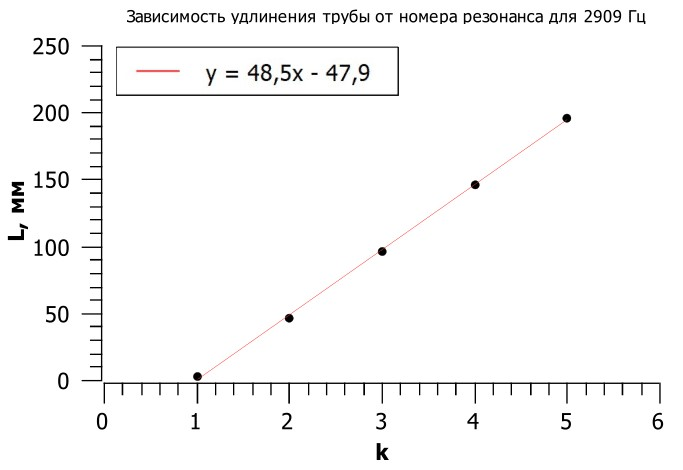
\includegraphics[width=60mm]{CO2_1-1.jpg}
&
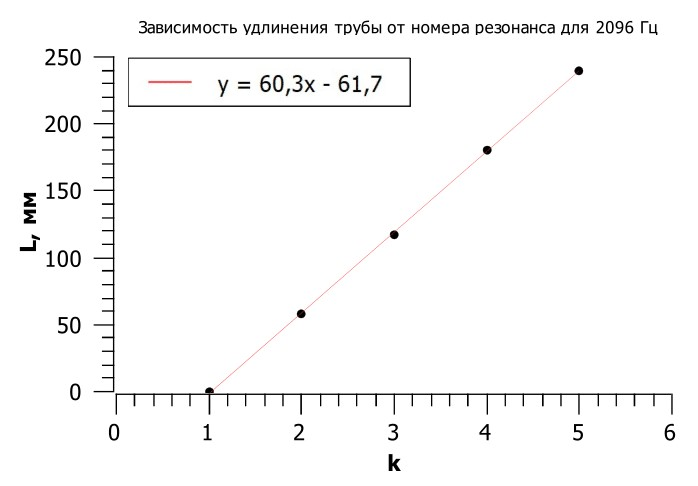
\includegraphics[width=60mm]{CO2_2-1.jpg}
\end{tabular}
\caption{Графики для углекислого газа}
\end{figure}

\begin{figure}[ht]\center
\begin{tabular}{cc}
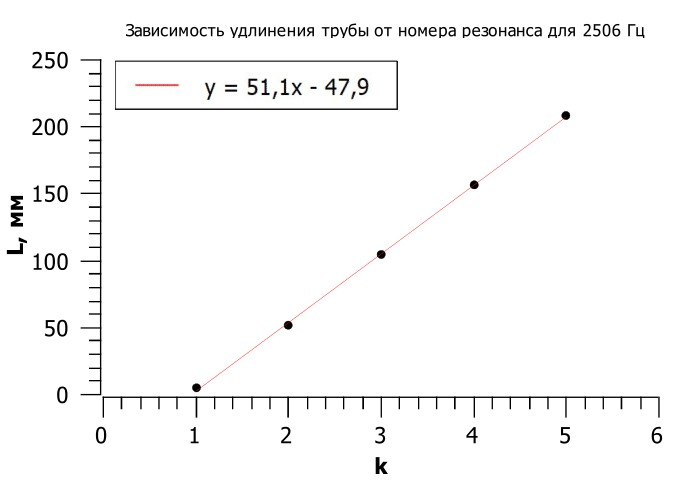
\includegraphics[width=60mm]{CO2_3-1.jpg}
&
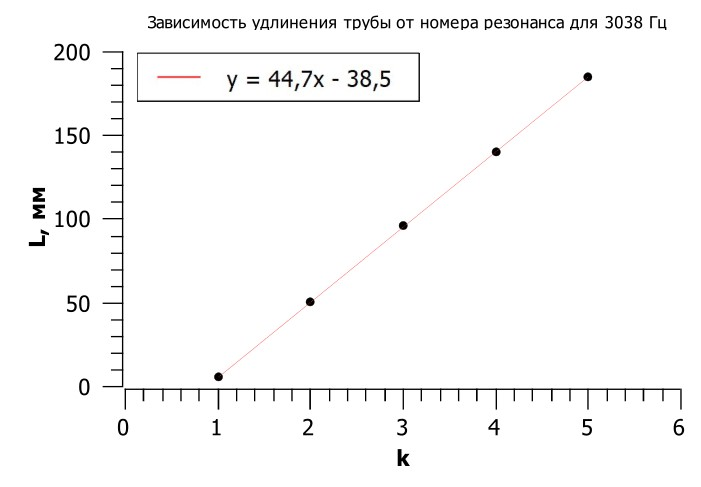
\includegraphics[width=60mm]{CO2_4-1.jpg}
\end{tabular}
\caption{Графики для глекислого газа}
\end{figure}

\vspace{0.5cm}

В качестве погрешностей будем учитывать только погрешность коэффициента в МНК, так как погрешности измерений достаточно малы:

\[\sigma_L = 0,5 \: \textit{мм} \quad \varepsilon_L = \sigma_L / L = 0,5 / 700 = 0,07\%\]

\[\sigma_f = 1 \: \textit{Гц} \quad \varepsilon_{f-max} = \sigma_f / f = 1 / 3000 = 0,03\%\]

В таком случае погрешность определения скорости звука будет определяться только погрешностью коэффициента  $b$. Посчитаем скорость звука, для каждого графика:

\[c_{2909} = 2 \cdot b_{2909} \cdot f_1 / 1000 = 2 \cdot 48,5 \cdot 2909 /1000 = 282,2 \: \textit{м}/\textit{с} \]

\[c_{2096} = 2 \cdot b_{2096} \cdot f_2 / 1000 = 2 \cdot 60,3 \cdot 2096 /1000 = 252,8 \: \textit{м}/\textit{с} \]

\[c_{2506} = 2 \cdot b_{2506} \cdot f_3 / 1000 = 2 \cdot 51,1 \cdot 2506 /1000 = 256,1 \: \textit{м}/\textit{с} \]

\[c_{3038} = 2 \cdot b_{3038} \cdot f_4 / 1000 = 2 \cdot 44,7 \cdot 3038 /1000 = 271,6 \: \textit{м}/\textit{с} \]

\[\sigma_{c_{2909}} = 0,54  \: \textit{м}/\textit{с}\]

\[\sigma_{c_{2096}} = 0,44  \: \textit{м}/\textit{с}\]

\[\sigma_{c_{2506}} = 0,43  \: \textit{м}/\textit{с}\]

\[\sigma_{c_{3038}} = 0,08  \: \textit{м}/\textit{с}\]

\vspace{0.5cm}

Аналогично построим таблицу для воздуха:

\begin{tabular}{|c|c|c|c|}
\hline 
$f_1 = 3474 \: \textit{Гц}$ & $f_2 = 4052 \: \textit{Гц}$ & $f_3 = 5111 \: \textit{Гц}$ & $f_4 = 2890 \: \textit{Гц}$ \\ 
\hline 
$\vartriangle L, \: \textit{мм}$ & $\vartriangle L, \: \textit{мм}$ & $\vartriangle L, \: \textit{мм}$ & $\vartriangle L, \: \textit{мм}$ \\ 
\hline 
5 & 0 &05 & 0 \\ 
\hline 
48 & 40 & 34 & 40 \\ 
\hline 
99 & 81 & 69 & 81 \\ 
\hline 
148& 120 & 101& 120 \\ 
\hline 
198 & 160 & 135 & 160 \\ 
\hline
\end{tabular}

\vspace{0.5cm}

При помощи МНК посчитаем коэффциенты для уравнения вида $y = a + bx$. Построим графики:

\vspace{0.5cm}

\begin{figure}[ht]\center
\begin{tabular}{cc}
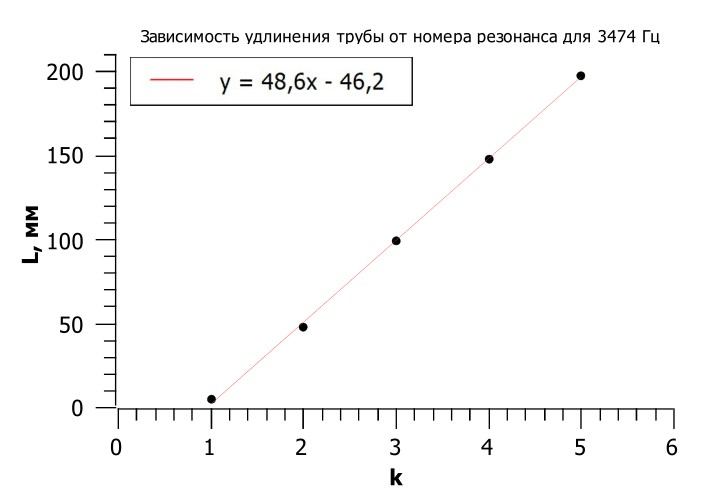
\includegraphics[width=60mm]{V_1-1.jpg}
&
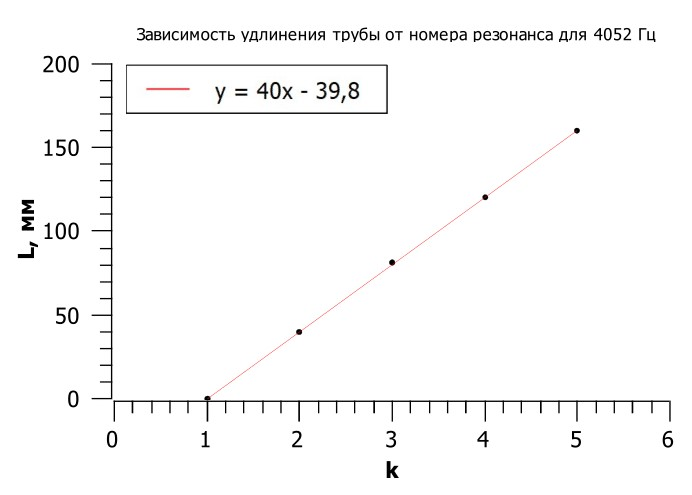
\includegraphics[width=60mm]{V_2-1.jpg}
\end{tabular}
\caption{Графики для воздуха}
\end{figure}

\begin{figure}[ht]\center
\begin{tabular}{cc}
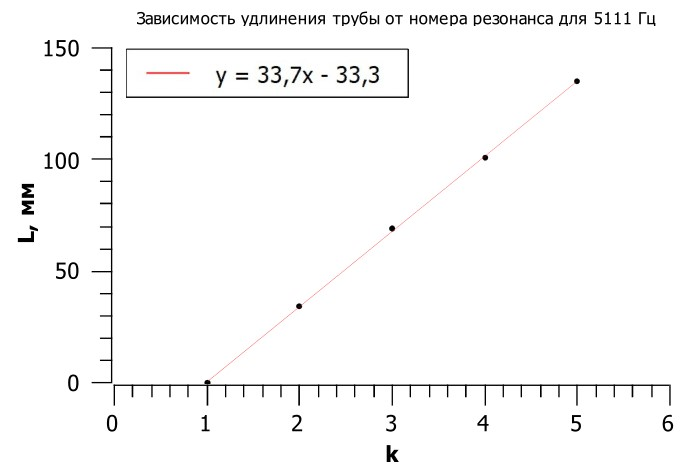
\includegraphics[width=60mm]{V_3-1.jpg}
&
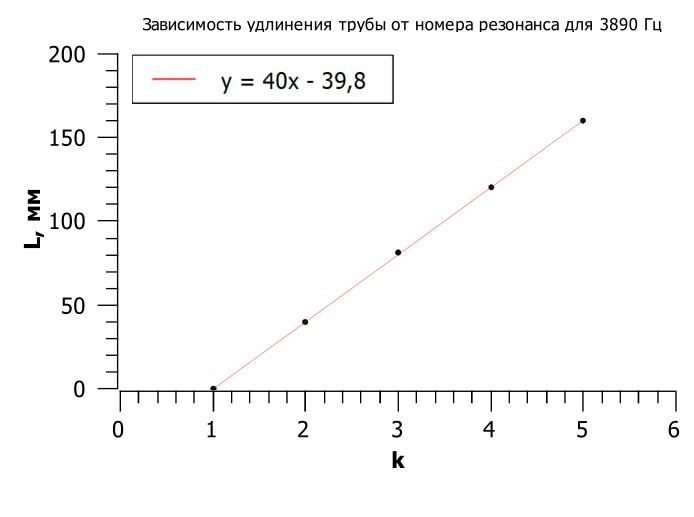
\includegraphics[width=60mm]{V_4-1.jpg}
\end{tabular}
\caption{Графики для воздуха}
\end{figure}

\vspace{0.5cm}

Погрешность, аналогично вычислениям для углекислого газа, будет вычисляться только по погрешности МНК. Посчитаем скорость звука, для каждого графика:

\[c_{3474} = 2 \cdot b_{3474} \cdot f_1 / 1000 = 2 \cdot 48,6 \cdot 3474 /1000 = 337,7 \: \textit{м}/\textit{с} \]

\[c_{4052} = 2 \cdot b_{4052} \cdot f_2 / 1000 = 2 \cdot 40,0 \cdot 4052 /1000 = 324,2 \: \textit{м}/\textit{с} \]

\[c_{5111} = 2 \cdot b_{5111} \cdot f_3 / 1000 = 2 \cdot 33,7 \cdot 5111 /1000 = 344,5 \: \textit{м}/\textit{с} \]

\[c_{3890} = 2 \cdot b_{3890} \cdot f_4 / 1000 = 2 \cdot 40,0 \cdot 3890 /1000 = 311,2 \: \textit{м}/\textit{с} \]

\[\sigma_{c_{3474}} = 0,59  \: \textit{м}/\textit{с}\]

\[\sigma_{c_{4052}} = 0,13  \: \textit{м}/\textit{с}\]

\[\sigma_{c_{5111}} = 0,19  \: \textit{м}/\textit{с}\]

\[\sigma_{c_{3890}} = 0,13  \: \textit{м}/\textit{с}\]

\vspace{0.5cm}

Значения полученные для скорости воздуха с высокой точностью совпадают с табличными. Для воздуха верно значение 340 \textit{м}/\textit{с}, а для углекислого газа 260 \textit{м}/\textit{с}. Определим среднее значение скорости звука из наших измерений:

\[c_{CO2\textit{ср}} = \frac{282,2 + 252,8 + 256,1 + 271,6}{4} = 265,7 \: \textit{м}/ \textit{с}\]

\[c_{V\textit{ср}} = \frac{337,7+324,4+344,5+311,2}{4} = 329,5 \: \textit{м}/ \textit{с}\]

За погрешность возьме максимальное значение погрешности для каждого газа:

\[\sigma_{c_{CO2}} = 0,54 \: \textit{м}/ \textit{с}\]

\[\sigma_{V} = 0,59 \: \textit{м}/ \textit{с}\]

\vspace{0.5cm}

Теперь, по формуле (\ref{1}) посчитаем значение показателя адиабаты в зависимости от температуры:

\[\gamma = \frac{\mu}{RT}c^2\]

$\mu_V$ возьмем равным 29 \textit{г}/\textit{моль}, $\mu_{CO2}$ возьмем равным 44 \textit{г}/\textit{моль} , а \textit{R} равным 8,31 \textit{Дж}/(\textit{моль}$\cdot$\textit{К}). 
Все измерения до этого момента проводились при температуре $T = 295,6 \: \textit{К}$, погрешность измерения температуры определяется характеристиками термометра и составляет: $\sigma_T = 0,1 \: \textit{К}$.

\[\gamma_{V-mv} = \frac{\mu_{V}}{R T_{295,6}}c_{V}^2 = \frac{0,029}{8,31 \cdot 295,6} \cdot 329,5^2 = 1,29\] 

\[\sigma_{\gamma_{V-mv}} = \gamma_{V-mv} \sqrt{\Big( \frac{\sigma_T}{T_{295,6}}\Big)^2 + \Big(2 \cdot \frac{\sigma_{c_{V}}}{c_{V} \Big)^2}} = 1,29 \sqrt{0,0003^2 + 0,0017^2} =  0,0022\]


\[\gamma_{CO2-mv} = \frac{\mu_{CO2}}{R T_{295,6}}c_{CO2}^2 = \frac{0,044}{8,31 \cdot 295,6} \cdot 265,7^2 = 1,26\] 

\[\sigma_{\gamma_{CO2-mv}} = \gamma_{CO2-mv} \sqrt{\Big( \frac{\sigma_T}{T_{295,6}}\Big)^2 + \Big(2 \cdot \frac{\sigma_{c_{CO2}}}{c_{CO2} \Big)^2}} = 1,26 \sqrt{0,0003^2 + 0,002^2} =  0,0025\]

\vspace{0.5cm}

Полученный показатель адиабаты для углекислого газа и воздуха отличаются от табличных значений на $7\%$, такое отличие, как я считаю, обусловлено трудностью поймать момент резонанса, когда каждый, даже малейший поворот ручки сдвигает значение частоты на значимую величину. В целом отличие от табличных значений не слишком большое, но измерение показателя адиабаты с более высокое точностью, по-моему мнению, требует либо другого метода, либо оборудования лишенного вышеназванного недостатка.

\textbf{2.} Проведем измерения для неподвижной трубы, длина трубы равна $L = 570 \: \textit{мм}$. Таблица для

\vspace{0.5cm}

\begin{tabular}{|c|c|c|c|c|c|c|c|c|}
\hline 
$f, \: \textit{Гц}$ & 1071 & 1280 & 1501 & 1712 & 1922 & 2312 & 2998 & 2805 \\ 
\hline
k  &  6  & 7 & 8 & 9 & 10 & 12 & 14 & 15\\
\hline
\end{tabular} 

\vspace{0.5cm}

\begin{tabular}{|c|c|c|c|c|c|c|c|c|}
\hline 
$f, \: \textit{Гц}$ & 1003 & 1322 & 1501 & 1673 & 1803 & 2350 & 2505 & 3159 \\ 
\hline 
k & 5 & 7 & 8 & 9 & 10 & 12 & 13 & 17 \\ 
\hline 
\end{tabular} 

\vspace{0.5cm}

По полученным данным при помощи МНК построим графики:

\vspace{0.5cm}

\begin{figure}[ht]\center
\begin{tabular}{cc}
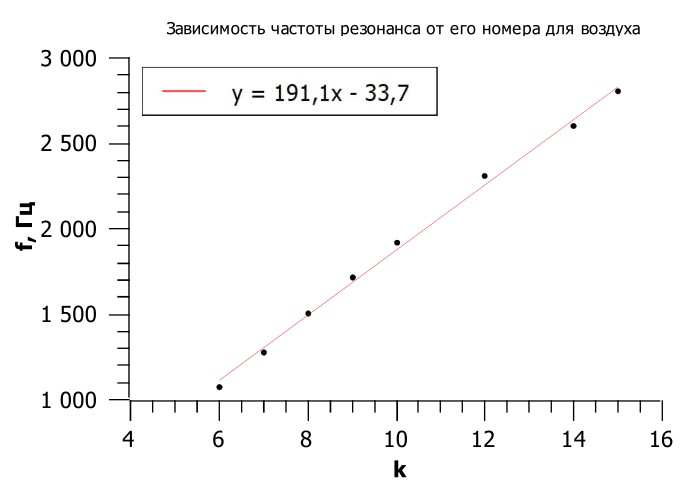
\includegraphics[width=60mm]{V_5-1.jpg}
&
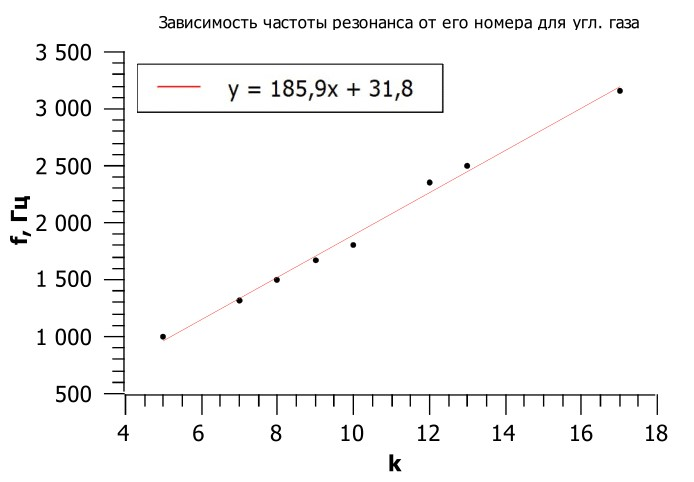
\includegraphics[width=60mm]{CO2_5-1.jpg}
\end{tabular}
\caption{Зависимость частоты резонанса от его номера для двух газов}
\end{figure}

\vspace{0.5cm}

По формуле (\ref{5}) можем найти скорость звука, умножив угловой коэффициент прямой (он посчитан в файле с вычислениями) на 2 длины трубы. Выпишем длину трубы и угловый коэффициенты:

\[L = 700 \: \textit{мм}, \quad \sigma_L = 5 \: \textit{мм}\]

\[k_{\textit{V}} = 191,1 \: \textit{Гц}, \quad \sigma_{k_{\textit{V}}} = 4,2 \: \textit{Гц}\]

\[k_{\textit{CO2}} = 185,9 \: \textit{Гц}, \quad \sigma_{k_{\textit{CO2}}} = 5,3 \: \textit{Гц}\]

\vspace{0.5cm}

И наконец найдем значение для скорости звука:

\[c_{V} = 2L \cdot k_{\textit{V}} = 2\cdot 0,7 \cdot 191,1 = 267,5 \: \textit{м}/ \textit{с}\]

\[\sigma_{c_{V}} = c_{V} \cdot \sqrt{\Big( \frac{\sigma_L}{L} \Big)^2 + \Big( \frac{\sigma_{k_{\textit{V}}}}{k_{\textit{V}}} \Big)^2} = 267,5 \sqrt{0,007^2 + 0,022^2} = 6,18 \: \textit{м}/ \textit{с}\]

\[c_{CO2} = 2L \cdot k_{\textit{V}} = 2\cdot 0,7 \cdot 185,9 = 260,3 \: \textit{м}/ \textit{с}\]

\[\sigma_{c_{CO2}} = c_{CO2} \cdot \sqrt{\Big( \frac{\sigma_L}{L} \Big)^2 + \Big( \frac{\sigma_{k_{\textit{CO2}}}}{k_{\textit{CO2}}} \Big)^2} = 260,3 \sqrt{0,007^2 + 0,029^2} = 7,76 \: \textit{м}/ \textit{с}\]

\vspace{0.5cm}

Заметим, что значение скорости звука для воздуха не совпадает с табличным и больше похоже на значение скорости звука для углекислого газа. Это может быть вызвано тем, что труба не была хорошо прочищена после того, как на ней поработали с воздухом. Следовательно этому значение не стоит доверять.

Данные углекислого газа совпадают с полученными ранее данными и табличным значением. Погрешность также не очень велика и составляет около $3\%$ от полученной величины.

Так как данные измерения проводились лишь для проверки того, насколько точно была измерена скорость звука, для полученнных значений показатель адиабаты я находить не буду(к тому же в следующих опытах будет получен показатель адиабаты по схожему методу).

\vspace{0.5cm}

\textbf{3.} Теперь пересядем на 2 установку и будем измерять скорость звука, оставляя постоянной длину трубы, но меняя температуру газа и частоту звукового генератора. Запишем измеренные данные в таблицу, всего таблицу.

\begin{tabular}{|c|c|c|c|c|}
\hline 
k & $f, \: \textit{Гц}$ (303,2 \textit{К}) & $f, \: \textit{Гц}$ (313,2 \textit{К}) & $f, \: \textit{Гц}$ (323,2 \textit{К}) & $f, \: \textit{Гц}$ (333,2 \textit{К}) \\ 
\hline 
1 & 256 & 267 & 270 & 275 \\ 
\hline 
2 & 502 & 514 & 520 & 524 \\ 
\hline 
3 & 752 & 768 & 773 & 780 \\ 
\hline 
4 & 1005 & 1024 & 1034 & 1027 \\ 
\hline 
5 & 1246 & 1280 & 1283 & 1301 \\ 
\hline 
\end{tabular} 

\vspace{0.5cm}

При помощи МНК построим графики:

\begin{figure}[h!]
\centering
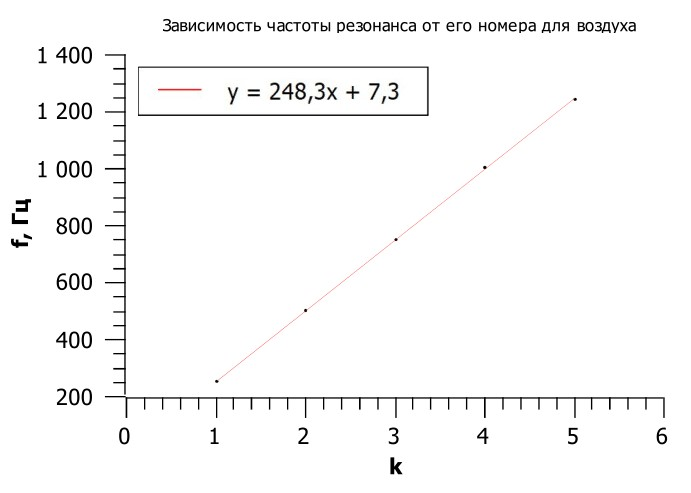
\includegraphics[scale=0.4]{V_6-1.jpg}
\caption{T = 303,2 К}
\label{fig:Experimental setup}
\end{figure}

\begin{figure}[h!]
\centering
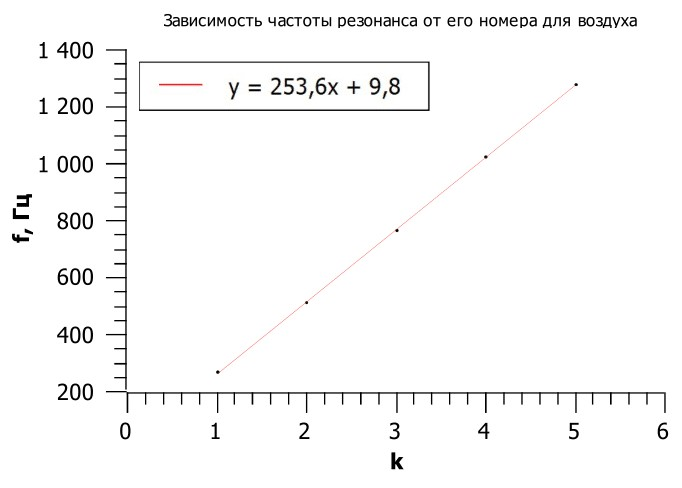
\includegraphics[scale=0.4]{V_7-1.jpg}
\caption{T = 313,2 К}
\label{fig:Experimental setup}
\end{figure}


\begin{figure}[h!]
\centering
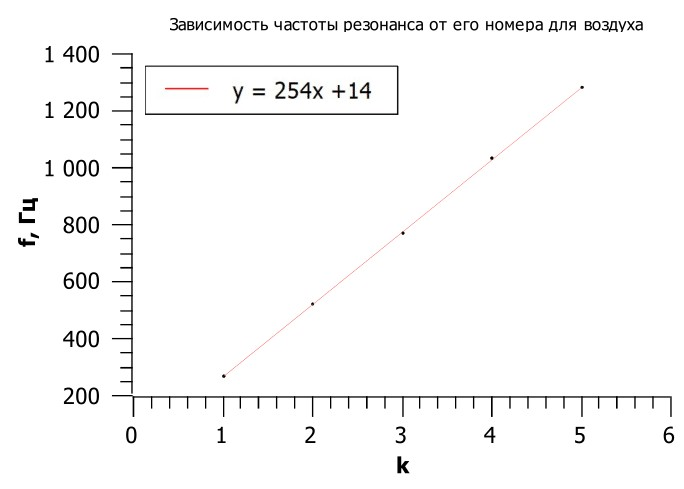
\includegraphics[scale=0.4]{V_8-1.jpg}
\caption{T = 323,2 К}
\label{fig:Experimental setup}
\end{figure}

\begin{figure}[h!]
\centering
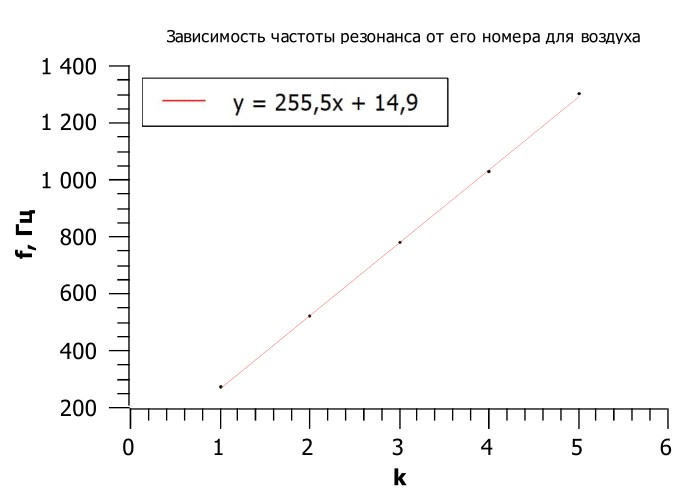
\includegraphics[scale=0.4]{V_9-1.jpg}
\caption{T = 333,2 К}
\label{fig:Experimental setup}
\end{figure}

\vspace{0.5cm}

Взяв посчитанные коэффициенты из документа с вычислениями, посчитаем по формуле (\ref{5}) значение скорости звука:

\[L = 700 \: \textit{мм}, \quad \sigma_L = 5 \: \textit{мм}\]

\[k_{303,2} = 248,3 \: \textit{Гц}, \quad \sigma_{k_{303,2}} = 0,79 \: \textit{Гц}\]

\[k_{313,2} = 253,6 \: \textit{Гц}, \quad \sigma_{k_{313,2}} = 0,82 \: \textit{Гц}\]

\[k_{323,2} = 254,0 \: \textit{Гц}, \quad \sigma_{k_{323,2}} = 0,83 \: \textit{Гц}\]

\[k_{333,2} = 255,5 \: \textit{Гц}, \quad \sigma_{k_{353,2}} = 1,99 \: \textit{Гц}\]

\[с_{303,2} = 2L \cdot k_{303,2} = 2 \cdot 0,7 \cdot 248,3 = 347,6 \: \textit{м} / \textit{с}\]

\[\sigma_{c_{303,2}} = c_{303,2} \cdot \sqrt{\Big( \frac{\sigma_{k_{303,2}}}{k_{303,2}}\Big) ^2 + \Big( \frac{\sigma_L}{L}\Big) ^2} = 347,6 \cdot \sqrt{0,003^2 + 0,007^2} = 2,65 \: \textit{м} / \textit{с}\]

\[с_{313,2} = 2L \cdot k_{313,2} = 2 \cdot 0,7 \cdot 253,6 = 355,0 \: \textit{м} / \textit{с}\]

\[\sigma_{c_{313,2}} = c_{313,2} \cdot \sqrt{\Big( \frac{\sigma_{k_{313,2}}}{k_{313,2}}\Big) ^2 + \Big( \frac{\sigma_L}{L}\Big) ^2} = 355,0 \cdot \sqrt{0,003^2 + 0,007^2} = 2,7 \: \textit{м} / \textit{с}\]

\[с_{323,2} = 2L \cdot k_{323,2} = 2 \cdot 0,7 \cdot 254,0 = 355,6 \: \textit{м} / \textit{с}\]

\[\sigma_{c_{323,2}} = c_{323,2} \cdot \sqrt{\Big( \frac{\sigma_{k_{323,2}}}{k_{323,2}}\Big) ^2 + \Big( \frac{\sigma_L}{L}\Big) ^2} = 355,6 \cdot \sqrt{0,003^2 + 0,007^2} = 2,71 \: \textit{м} / \textit{с}\]

\[с_{333,2} = 2L \cdot k_{333,2} = 2 \cdot 0,7 \cdot 255,5 = 357,7 \: \textit{м} / \textit{с}\]

\[\sigma_{c_{333,2}} = c_{333,2} \cdot \sqrt{\Big( \frac{\sigma_{k_{333,2}}}{k_{333,2}}\Big) ^2 + \Big( \frac{\sigma_L}{L}\Big) ^2} = 357,7 \cdot \sqrt{0,008^2 + 0,007^2} = 3,8 \: \textit{м} / \textit{с}\]

\vspace{0.5cm}

В результате получились вполне правдоподобные значения. Также можно заметить, что с увеличением температуры, скорость звука также увеличивается, этот факт совпадает с теорией. 

Теперь, по формуле (\ref{1}) посчитаем значение показателя адиабаты в зависимости от температуры:

\[\gamma = \frac{\mu}{RT}c^2\]

$\mu$ возьмем равным 29 \textit{г}/\textit{моль}, а \textit{R} равным 8,31 \textit{Дж}/(\textit{моль}$\cdot$\textit{К}).

\[\gamma_{303,2} = \frac{\mu}{R T_{303,2}}c_{303,2}^2 = \frac{0,029}{8,31 \cdot 303,2} \cdot 347,6^2 = 1,39\] 

\[\sigma_{\gamma_{303,2}} = \gamma_{303,2} \sqrt{\Big( \frac{\sigma_T}{T_{303,2}}\Big)^2 + \Big(2 \cdot \frac{\sigma_{c_{303,2}}}{c_{303,2}} \Big)^2} = 1,39 \sqrt{0,0003^2 + 0,015^2} =  0,021\]

\[\gamma_{313,2} = \frac{\mu}{R T_{313,2}}c_{313,2}^2 = \frac{0,029}{8,31 \cdot 313,2} \cdot 355^2 = 1,4\] 

\[\sigma_{\gamma_{313,2}} = \gamma_{313,2} \sqrt{\Big( \frac{\sigma_T}{T_{313,2}}\Big)^2 + \Big(2 \cdot \frac{\sigma_{c_{313,2}}}{c_{313,2}} \Big)^2} = 1,4 \sqrt{0,0003^2 + 0,015^2} =  0,021\]

\[\gamma_{323,2} = \frac{\mu}{R T_{323,2}}c_{323,2}^2 = \frac{0,029}{8,31 \cdot 323,2} \cdot 355,6^2 = 1,38\] 

\[\sigma_{\gamma_{323,2}} = \gamma_{323,2} \sqrt{\Big( \frac{\sigma_T}{T_{323,2}}\Big)^2 + \Big(2 \cdot \frac{\sigma_{c_{323,2}}}{c_{323,2}} \Big)^2} = 1,38 \sqrt{0,0003^2 + 0,015^2} =  0,021\]

\[\gamma_{333,2} = \frac{\mu}{R T_{333,2}}c_{333,2}^2 = \frac{0,029}{8,31 \cdot 333,2} \cdot 357,7^2 = 1,37\] 

\[\sigma_{\gamma_{333,2}} = \gamma_{333,2} \sqrt{\Big( \frac{\sigma_T}{T_{333,2}}\Big)^2 + \Big(2 \cdot \frac{\sigma_{c_{333,2}}}{c_{333,2}} \Big)^2} = 1,37 \sqrt{0,0003^2 + 0,021^2} =  0,029\]

\vspace{0.5cm}
Получившиеся значения довольно близки к табличным, что показывает, что данный метод немного точнее первого. Вообше можно считать, что табличные значения совпали с измеренными нами, так как они находятся в пределах погрешности наших измерений.

\vspace{0.5cm}

\textbf{Вывод.} Мы смогли с высокой точностью определить скорость звука и показатель адиабаты двумя различными методами в которых используется звуковой генератор. В целом второй метод мне показался чуть более точным и удобным, так как там вероятность пропустить момент резонанса меньше, что снижает вероятность моей ошибки.

\vspace{0.5cm}

\textbf{Контрольные вопросы.} 

1. Запишем волновое уравнение и его решение для одномерного, плоского распространения звуковой волны в воздухе. При этом величина смещения бесконечно малого элемента среды (воздуха), заключенного между координатой $x$ и координатой $x + \bigtriangleup x, \: u(x,t)$, в волне будет завичсеть от двух переменных: пространственной координаты $x$ и времени $t$.

Вводя плотность среды $\rho_0$ и изменение плотности в волне $\bigtriangleup \rho$, из условия сохранения массы элемента получаем

\[\rho_0 \bigtriangleup x = (\rho_0 + \bigtriangleup \rho)[x + \bigtriangleup x + u(x + \bigtriangleup x, t) - x - u(x,t)].\]

Разлагая смещение в ряд Тейлора, имеем

\[\rho_0 \bigtriangleup x = (\rho_0 + \bigtriangleup \rho_[\bigtriangleup x + (\partial u/ \partial x)\bigtriangleup x].\]

Отсюда, так как $\bigtriangleup \rho \ll \rho$ и, следовательно,$(\partial u/ \partial x) \ll 1$,

\[\bigtriangleup \rho \approx -\rho_0 (\partial u/ \partial x).\]

Второй закон Ньютона для элемента даеь

\[\rho_0 \bigtriangleup x \frac{\partial^2 u}{\partial t^2} = p(x,t) -  p(x + \bigtriangleup x, t) \approx - \frac{\partial \bigtriangleup p}{\partial x} \bigtriangleup x\]

Предполагая, что процесс изменения плотности в волне происходится быстро и теплообмен не успевает произойти, т.е. предполагая, что процесс распространения звука является адиабатическим, имеем

\[\bigtriangleup p = (\partial p/ \partial \rho)_{\textit{ад}} \bigtriangleup \rho = c_{\textit{зв}}  \rho\]

Следовательно:

\[c = \sqrt{\frac{dP}{d \rho}}\]

Заменим в уравнении Пуассона $PV^{\gamma} = const$ объем на плотность $\rho = m/V$, после чего получим $P = const \cdot \rho^{\gamma}. Тогда после логарифмирования и дифференцирования этого выражения имеем$

\[\frac{dP}{P} = \gamma \frac{d \rho}{\rho}, \quad \textit{или} \quad \Big( \frac{dP}{d \rho}\Big)_{\textit{адиаб}} = \gamma \frac{P}{\rho}\]

\vspace{0.5cm}

2. В выбранном диапазоне температур показатель адиабаты не зависит от температуры, так как теплоемкость газа при постоянном обьеме и далении на данном участке практически не меняются.

\vspace{0.5cm}

3. Вообще нет, так как при температуре в 1000 градусов по Цельсию начнется переход газа в состояния называемое плазмой. Но в целом, изменение показателя адиабаты воздуха по сравнение с комнатной температурой нельзя будет назвать значительным. По табличным данным, показатель адиабаты изменится менее, чем на $3 \%$.

\end{document}